% Positron Emission tomography (includes Physics, detector basics, Event types and data types, PET ring systems and acquisition modes (2D and 3D) , Corrections, , PET WB acquisition mode and fussion -> multibed, Hybrid PET systems (PET-CT, PET-MR)) 
This section covers aspects of the main principles of \gls{pet} and serves as a brief introduction to the notions that are necessary for the description of the work carried out in this thesis. It is not an exhaustive review of the processes involved in \gls{pet} imaging. Readers can find more basic principles explained in detail in the textbooks which are frequently referenced in this chapter.

\section{Historical Perspective}
The main principles of a \Gls{pet} imaging system were developed and demonstrated with a working scanner prototype in the late 1970s by Ter-Pogossian et al.~\cite{Ter-Pogossian1975} and Phelps et al.~\cite{Phelps1975}. The main concept of their prototype, which forms the basis of \gls{pet} devices, was the placement of detectors in a circular formation around the imaged object and the detection of annihilation photon pairs which serves as "Electronic" collimation. This principle of "Electronic" collimation makes \gls{pet} imaging superior to single photon based imaging devices still until today as it does not require a physical collimator which considerably reduces the sensitivity, as in \gls{spect} imaging systems.
Early \gls{pet} systems were limited due to the cost and engineering limitations to an axial coverage of a few axial planes and were mostly used in brain imaging. Development of scanner models with a larger diameter and larger axial \gls{fov} enabled use for imaging of other organs than the brain~\cite{Nutt2002}.
The expanded \gls{fov} along with the capability of achieving whole-body coverage by use of shifted axial acquisitions~\cite{Dahlbom1992} (multiple axial bed positions to achieve whole-body coverage) have established the use of \gls{pet} in oncology~\cite{Bomanji2001} and driven many more technological developments towards higher sensitivity for improved small lesion detectability and reduction of scan time~\cite{Jones2017}.


\section{Fundamental physics of PET}

\subsection{Positron emission}
As its name suggests, \gls{pet} is an imaging method based on positron emission. Positron emission is a spontaneous process that happens as part of the β$^{+}$ decay process of radionuclides. 
Radionuclides are comprised of atoms with excess energy that decay to stable forms via routes that result in the emission of radiation.
The rate at which a radionuclide undergoes decay depends on its characteristic half-life $T_{1/2}$. This is defined as the time taken for half of the nuclei of a specific radionuclide to decay. The rate of decay at any time $t$ is defined as the activity $A(t)$, measured in Becquerels (Bq), which changes over time according to
\begin{equation} \label{Decay}
A(t) = A_0 e^{-\lambda t} \ ,
\end{equation}
where $A_0$ is the activity at reference time $t_0=0$ and $\lambda$ is the decay constant, for which 
\begin{equation} \label{Decayconstant}
\lambda = \frac{ln(2)}{T_{1/2}} \ .
\end{equation}
%
The β$^{+}$ decay process results in the emission of a positron (e$^{+}$) particle and a neutrino (ν). The positron is given part of the excess radioisotope energy in the form of kinetic energy, which when emitted within a material is gradually lost from continuous interactions with other atoms of the material until the positron approaches close to a rest. During this period the positron follows a tortuous random path. The positron range can be defined for a sufficiently large number of emissions as either the FWHM or the mean of the distribution of distances between the emission and annihilation positions. The positron range value will depend on the positrons energy spectrum and the interacting material properties. After most of its kinetic energy has been expended, the positron rapidly interacts with an electron and annihilates. This interaction results in the conversion of the two particles into two photons of 511 \si{k\electronvolt} which are emitted in almost opposite directions ($\sim$180$^{\circ}$). Due to the non-zero kinetic energy during the annihilation, the excess energy results in a small acollinearity of the photon pair. For \textit{in vivo} [$^{18}$F]-\gls{fdg} imaging, a common radiolabeled tracer used in PET oncology applications, it has been shown that the FWHM acollinearity is approximately 0.54$^{\circ}$~\cite{Shibuya2007}.
%
A list of positron emitting radionuclides which are commonly used in \gls{pet} imaging is given in table~\ref{tab:radioisotopes} along with relevant characteristics for PET imaging.

\begin{table}[htbp]
  \caption{Commonly used radioisotopes and their relevant characteristics for PET imaging~\cite{Conti2016}.}
\makebox[\textwidth][c]{
    \begin{tabular}{cccc}
\toprule
  Radionuclide & Half-life & \multicolumn{1}{c}{ e$^{+}$ maximum energy (\si{M\electronvolt})} & \multicolumn{1}{c}{Mean range in water (mm)} \\
\midrule
\ce{^15O} & 2 min & 1.732 &  3.0    \\
\ce{^13N} & 10.0 min & 1.199  & 1.8  \\
\ce{^11C} & 20.4 min & 0.96 & 1.2   \\
\ce{^18F} & 110 min & 0.634 &  0.6  \\
\ce{^68Ga} & 67.8 min & 1.899 &2.9      \\
\ce{^64Cu} & 12.7 h & 0.653 &  0.7  \\
\ce{^89Zr} & 78.4 h& 0.902 & 1.3    \\
\bottomrule
\end{tabular}%
}
\label{tab:radioisotopes}%
\end{table}%

\subsection{Interactions with matter}
The mean range of positrons from commonly used PET radionuclides is in the order of a few millimetres within tissue and almost all positrons are annihilated within the body.
On the other hand, the 511 \si{k\electronvolt} photons have fewer chances of interacting within the body and a large fraction of them will exit the imaged object without interacting. 

The two most probable interactions for photons of 511 \si{k\electronvolt} in tissue are photoelectric absorption and Compton scattering. In photoelectric absorption, the photon is completely absorbed while interacting with an atomic electron of the inner shell, to which it provides all of its energy. In Compton scattering, the photon interacts with an atomic electron of an outer shell, to which it passes part of its energy. This scattering process results in a change of direction and reduction of the energy of the original photon, while the loosely bound electron is ejected from the interacting atom. Between the two processes, the Compton effect is the dominant interaction for 511 \si{k\electronvolt} photons in tissue. Elastic scattering (Rayleigh scattering) is another interacting process in which no loss of energy occurs and the direction of the incident photon is changed by a relatively small angle. This interaction is more dominant in lower energies than 511 \si{k\electronvolt} photons.
%
\begin{figure} [h!]
\centering
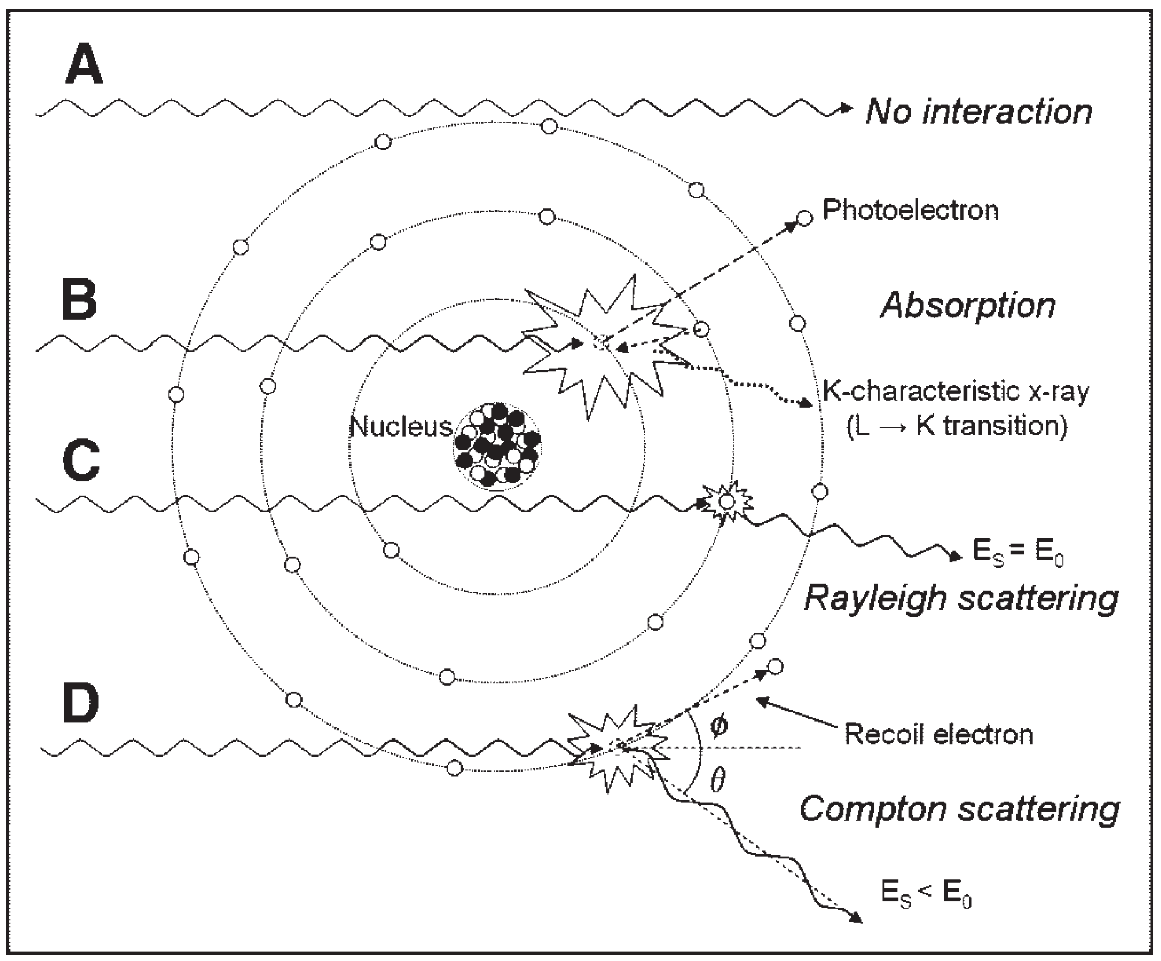
\includegraphics[scale=0.45,angle=0]{2_Theory_Methods/figures/Interactions.pdf}
\caption{Illustration of the described interactions. (A) No interaction resulting in transmission of photon. (B) Photoelectric absorption from inner shell electron, resulting in its ejection and followed by an inner electron transition and characteristic X-Ray emission. (C) Elastic (Rayleigh) scattering conserving the energy of the photons but resulting in small angle change in direction. (D) Compton scattering with outer shell electron resulting to change of energy and direction of incident photon. Adapted from \textit{Seibert et al.}~\cite{Seibert2005}.} 
\label{fig_2:511_interactions}
\end{figure} 
%
\subsection{Attenuation}
Knowledge of the probabilities for the interaction of 511 \si{k\electronvolt} photons in a material can be used to calculate a precise attenuation factor that can be applied at the macroscopic level. Given a well collimated photon beam of intensity $I_0$, the intensity $I_x$ at depth $x$ within the material (along the direction of the beam) will be reduced due to interactions with the material according to Beer-Lambert's law
\begin{equation} \label{Attenuation}
I_x = I_0 e^{-\mu x} \ ,
\end{equation}
where $\mu$ is the linear attenuation coefficient (in cm$^{-1}$). This factor accounts for all possible interactions, whether absorption or scattering, and its value depends on the material properties and the energy of the photons.
%
%Specifically for \gls{pet} where we are interested in the detection of both annihilation photons, the attenuation in the direction of the photon pair can be summed up, resulting in a factor that is independent of the depth of the annihilation and is only depended of the attenuation coefficient of the tissues or materials crossed by the line connecting the two photon detections and the total length of the line within the body, as shown in figure~\ref{fig_2:511_attenuation}~\cite{Phelps1975}. 
%
%\begin{figure} [h!]
%\centering
%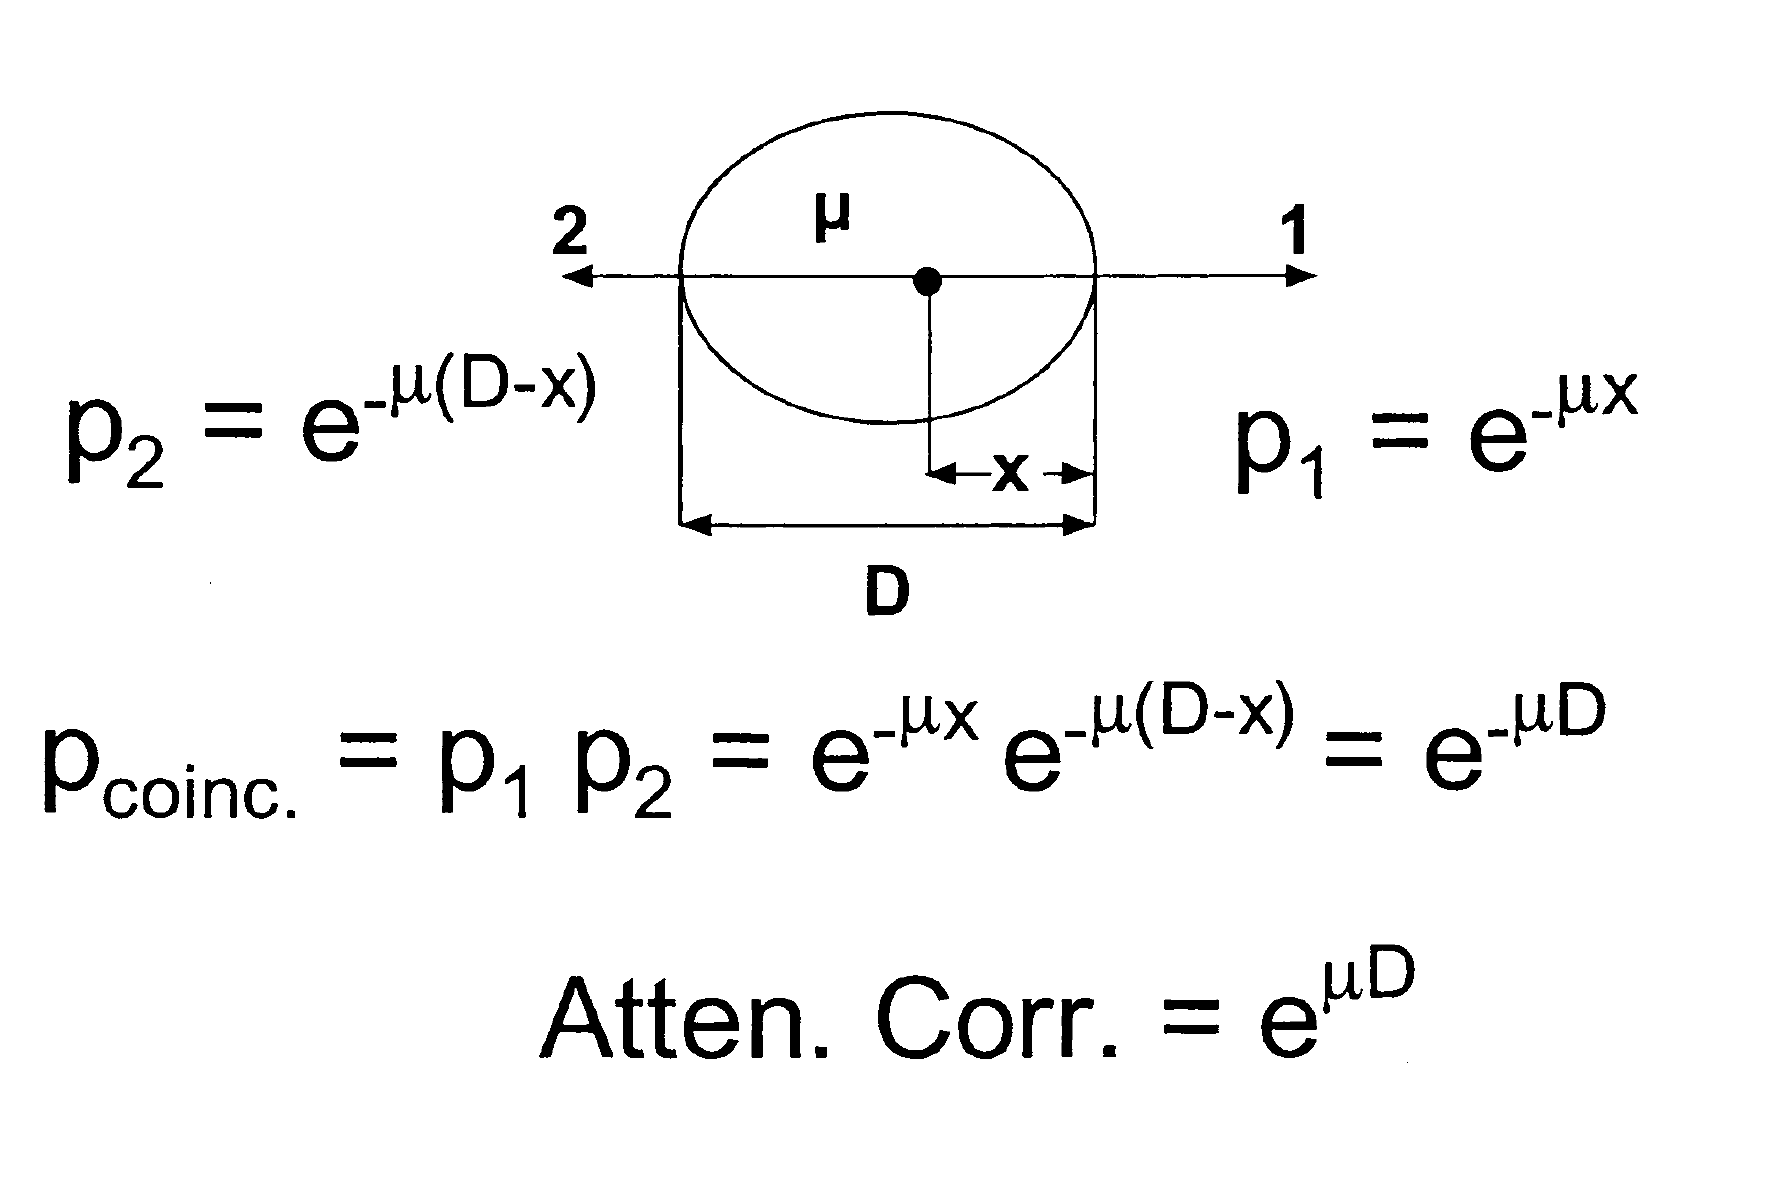
\includegraphics[scale=0.45,angle=0]{2_Theory_Methods/figures/Phelps_LOR_attenuation_correction.png}
%\caption{Attenuation of LORs TODO:  to include in text ! } 
%\label{fig_2:511_attenuation}
%\end{figure} 
%
\section{PET Systems}

\subsection{PET Detectors}
The goal of a PET imaging system is to stop and detect the annihilation photon pairs and record information that can be used to estimate the annihilation event's position.
The basic component for the detection of annihilation gammas is the scintillation crystal. These are inorganic crystals that emit light (lower energy photons) upon interaction with the gammas. The amount of produced light is proportional to the energy deposited by the gamma interactions and can be used to deduce energy information of the interaction. Photosensitive detectors are coupled with the crystals to capture the produced light and output an electronic signal that can be digitally registered. Traditionally \glspl{pmt} are used in most PET systems, while some more recent systems make use of \glspl{sipm}. Depending on their mode of operation \glspl{sipm} can allow for better efficiency and response speed and can be used in conditions where \glspl{pmt} could not, such as within the MR field of PET-MR hybrid systems. More details on \gls{sipm} integration in PET/MR are given in section~\ref{sec:PET_MR_Systems}.
%
%\footnotetext{https://www.radiologycafe.com/radiology-trainees/frcr-physics-notes/pet-imaging}
\begin{figure} [h!]
\centering
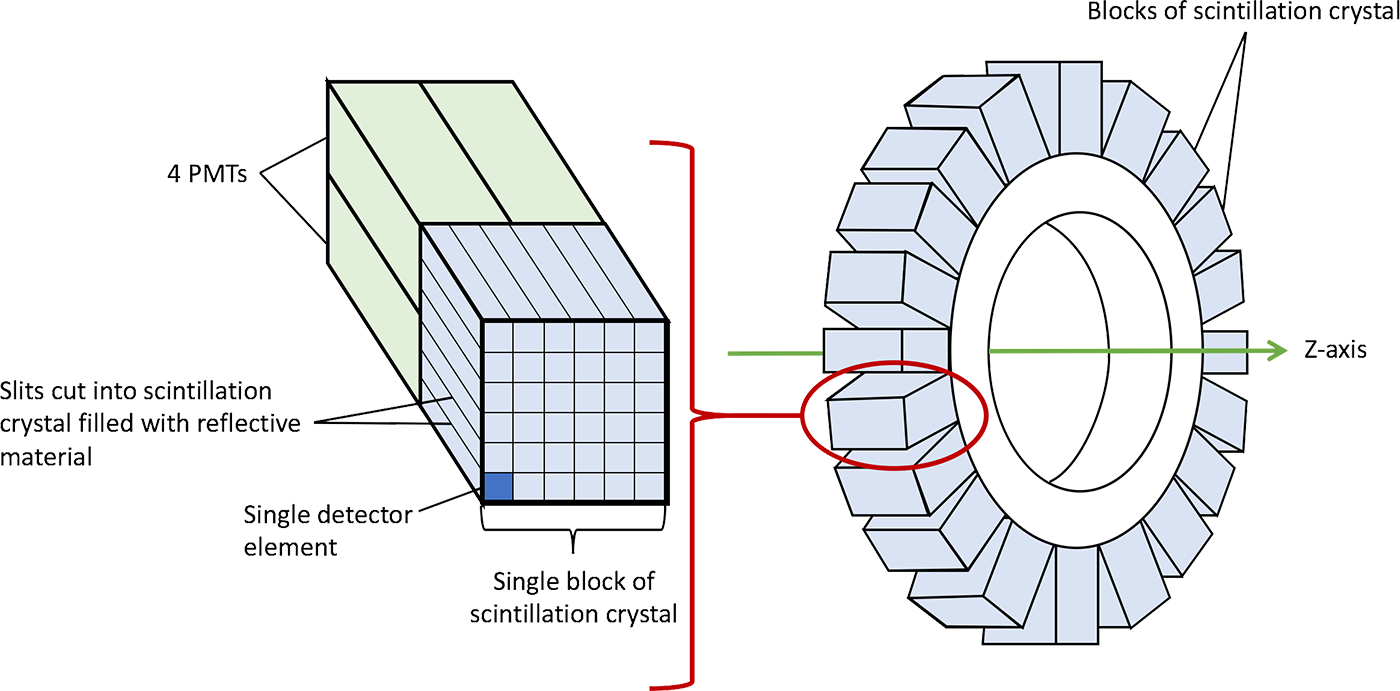
\includegraphics[scale=0.28,angle=0]{2_Theory_Methods/figures/block_detector.png}
\caption{Example illustration of PMT based block detector diagram and their placement within a PET ring (Adapted from www.radiologycafe.com) } 
\label{fig_2:BlockDetectorAndRing}
\end{figure} 
%\begin{figure} [h!]
%\centering
%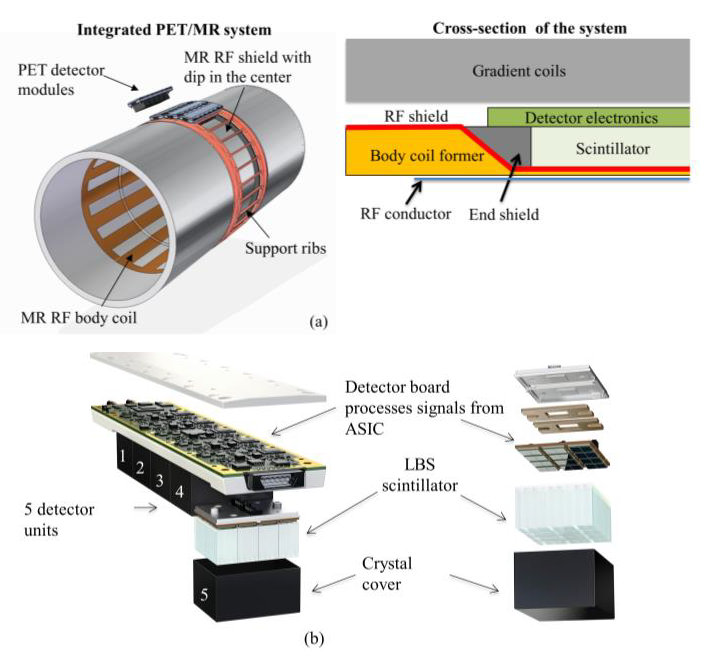
\includegraphics[scale=0.45,angle=0]{2_Theory_Methods/figures/SignaPETMR_Integrated_System.png}
%\caption{Schematic of an hybrid PET-MR system with, comprising of detector module units (bottom) in a ring formation within the MR RF body coil (top)~\cite{Levin2016}.} 
%\label{fig_2:SignaPETMR_Integrated_System}
%\end{figure} 
%%
%
The most common configuration of the PET detectors is within a block or module configuration, where a smaller number of photosensitive detectors to crystals is used. An example of a single crystal block to 4 \glspl{pmt} is shown in figure~\ref{fig_2:BlockDetectorAndRing} for PMT based scanners. The crystals are partially cut into segments to reduce lateral dispersion of light and improve localisation of detection by the \glspl{pmt}. In the example of figure~\ref{fig_2:BlockDetectorAndRing} the crystal is cut in a 6$\times$6 configuration.

The blocks or modules are placed in ring configurations that provide full 360$^{\circ}$ of coverage in the transaxial direction. Multiple rings are often placed adjacent to each together to increase axial coverage and solid angle coverage which provides increased detection sensitivity. 

\subsection{PET Data coincidence sorting}
Individual events recorded by the detectors are called \textit{single} events. In \gls{pet}, detection of annihilation events requires the detection of both annihilation generated photons. To identify these photons the detection system makes use of "coincidence detection". Pairs of single events detected within a predefined timing window are assumed to be photons originating from a single annihilation which are defined as \textit{prompt coincidence events}.
The line connecting the two detectors that record the coincident event is defined as the \gls{lor}.

Improved timing resolution of detector systems has enabled for further information of the annihilation point to be made by capturing the detector arrival difference of the two annihilation photons. This difference can help localise the point on the \gls{lor} where the annihilation took place, within some range of uncertainty defined by the detector timing resolution. This capability of PET is referred to as \textit{time-of-flight} (TOF).
This information, collected for each coincidence event, can then be used within the image reconstruction process for improved results, as it will be shortly described in chapter~\ref{Chap2_3:Reconstruction}.

\begin{figure} [h!]
\centering
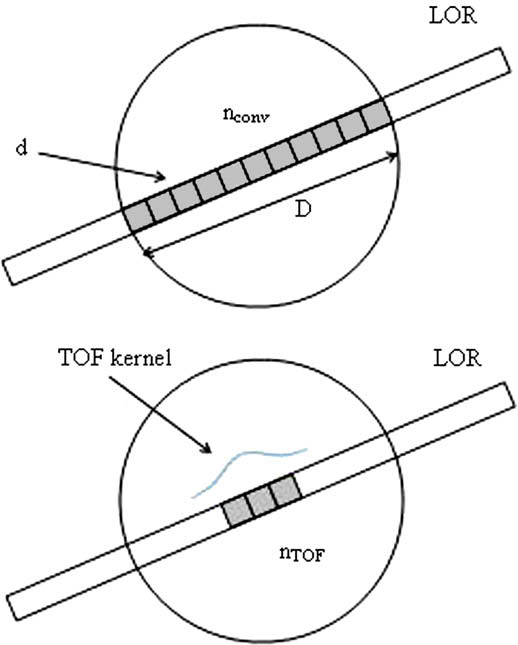
\includegraphics[scale=0.55,angle=0]{2_Theory_Methods/figures/TOF_bin.png}
\caption{Illustration of non-TOF (top) and TOF (bottom) information regarding the annihilation event's position across an LOR~\cite{Conti2009}.} 
\label{fig_2:TOF_bin}
\end{figure} 
%
Unfortunately not all coincidence events recorded within the coincidence window will always be originating from the same annihilation event. Apart from true coincidences, they could also be one of the following type of events. 
%
\begin{itemize}
\item\textbf{Random event}\\
As the rate of single events increases the chances of photons originating from different annihilation events being detected within the coincidence timing window are also increasing. These photons will not have interacted with the body before being detected.
In this case, the system will record coincidence events that are not correlated. These events are referred to as random events. 
The rate of random events is directly proportional to the size of the timing window and to the square of the activity in the scanner. These events are uncorrelated to the imaged object and hence degrade the acquired data and subsequently image quality and quantification.  
The expected rate of random coincidences can be estimated using the rates of single events or using delayed coincidence windows. These estimations are then pre-processed and subsequently applied as corrections in the image reconstruction process. 
Randoms estimations can be made using the rates of single events or using delayed coincidence windows, which can then be applied as corrections during the image reconstruction process. 
%
%Photons travelling in straight line (no interaction with the body)
%
\item\textbf{Scatter events}\\
As described scattering of the annihilation gammas results in changes to its energy and direction of travel. Subsequent detection of scattered gammas results in mispositioned \glspl{lor} that also degrade the data, image quality and quantification. 
Because scattered gammas have lower energy than 511 \si{k\electronvolt}, they can be rejected by applying a low energy threshold in the detectors. But due to energy resolution limitations, this threshold is set low enough to best avoid rejection of true coincidence events while still filtering a reasonable amount of scattered events.
To correct for the remaining events that are being recorded as true coincidences, special scatter simulation algorithms are employed to estimate the amount of scatter coincidences in the data and account for it during the image reconstruction process~\cite{Watson1996,Polycarpou2011}.
%
\item\textbf{Multiple events}\\
Multiple single events (more than two) can be recorded within the coincidence timing window in which case they are referred to as multiple events. As these cannot be used to resolve \glspl{lor}, they are either rejected completely or in some cases processed further to deduce which pair of single events are more likely to be true coincidences, using techniques that vary between scanner models and manufacturers. 
%
\item\textbf{Delayed event}\\
As described above, an estimation of randoms can be made using an additional detection channel to capture coincidences with a delay of several times the duration of the coincidence window. These events are considered uncorrelated and serve as a direct measurement of randoms. Specific variance reduction techniques are then applied on these randoms estimations before being used as corrections in reconstruction, to avoid inducing additional noise in the data~\cite{Bailey2005}.
%
\item\textbf{Prompt event}\\
True, random and scatter events that meet the acceptance criteria for coincidence detection are indistinguishable at the time of detection and recorded as valid coincidence events. They are referred to as prompt events.
These are pre-corrected or used directly in the reconstruction process along with the corrections, depending on the use of either analytical or statistical reconstruction methods respectively.
\end{itemize}
%
\begin{figure} [h!]
\centering
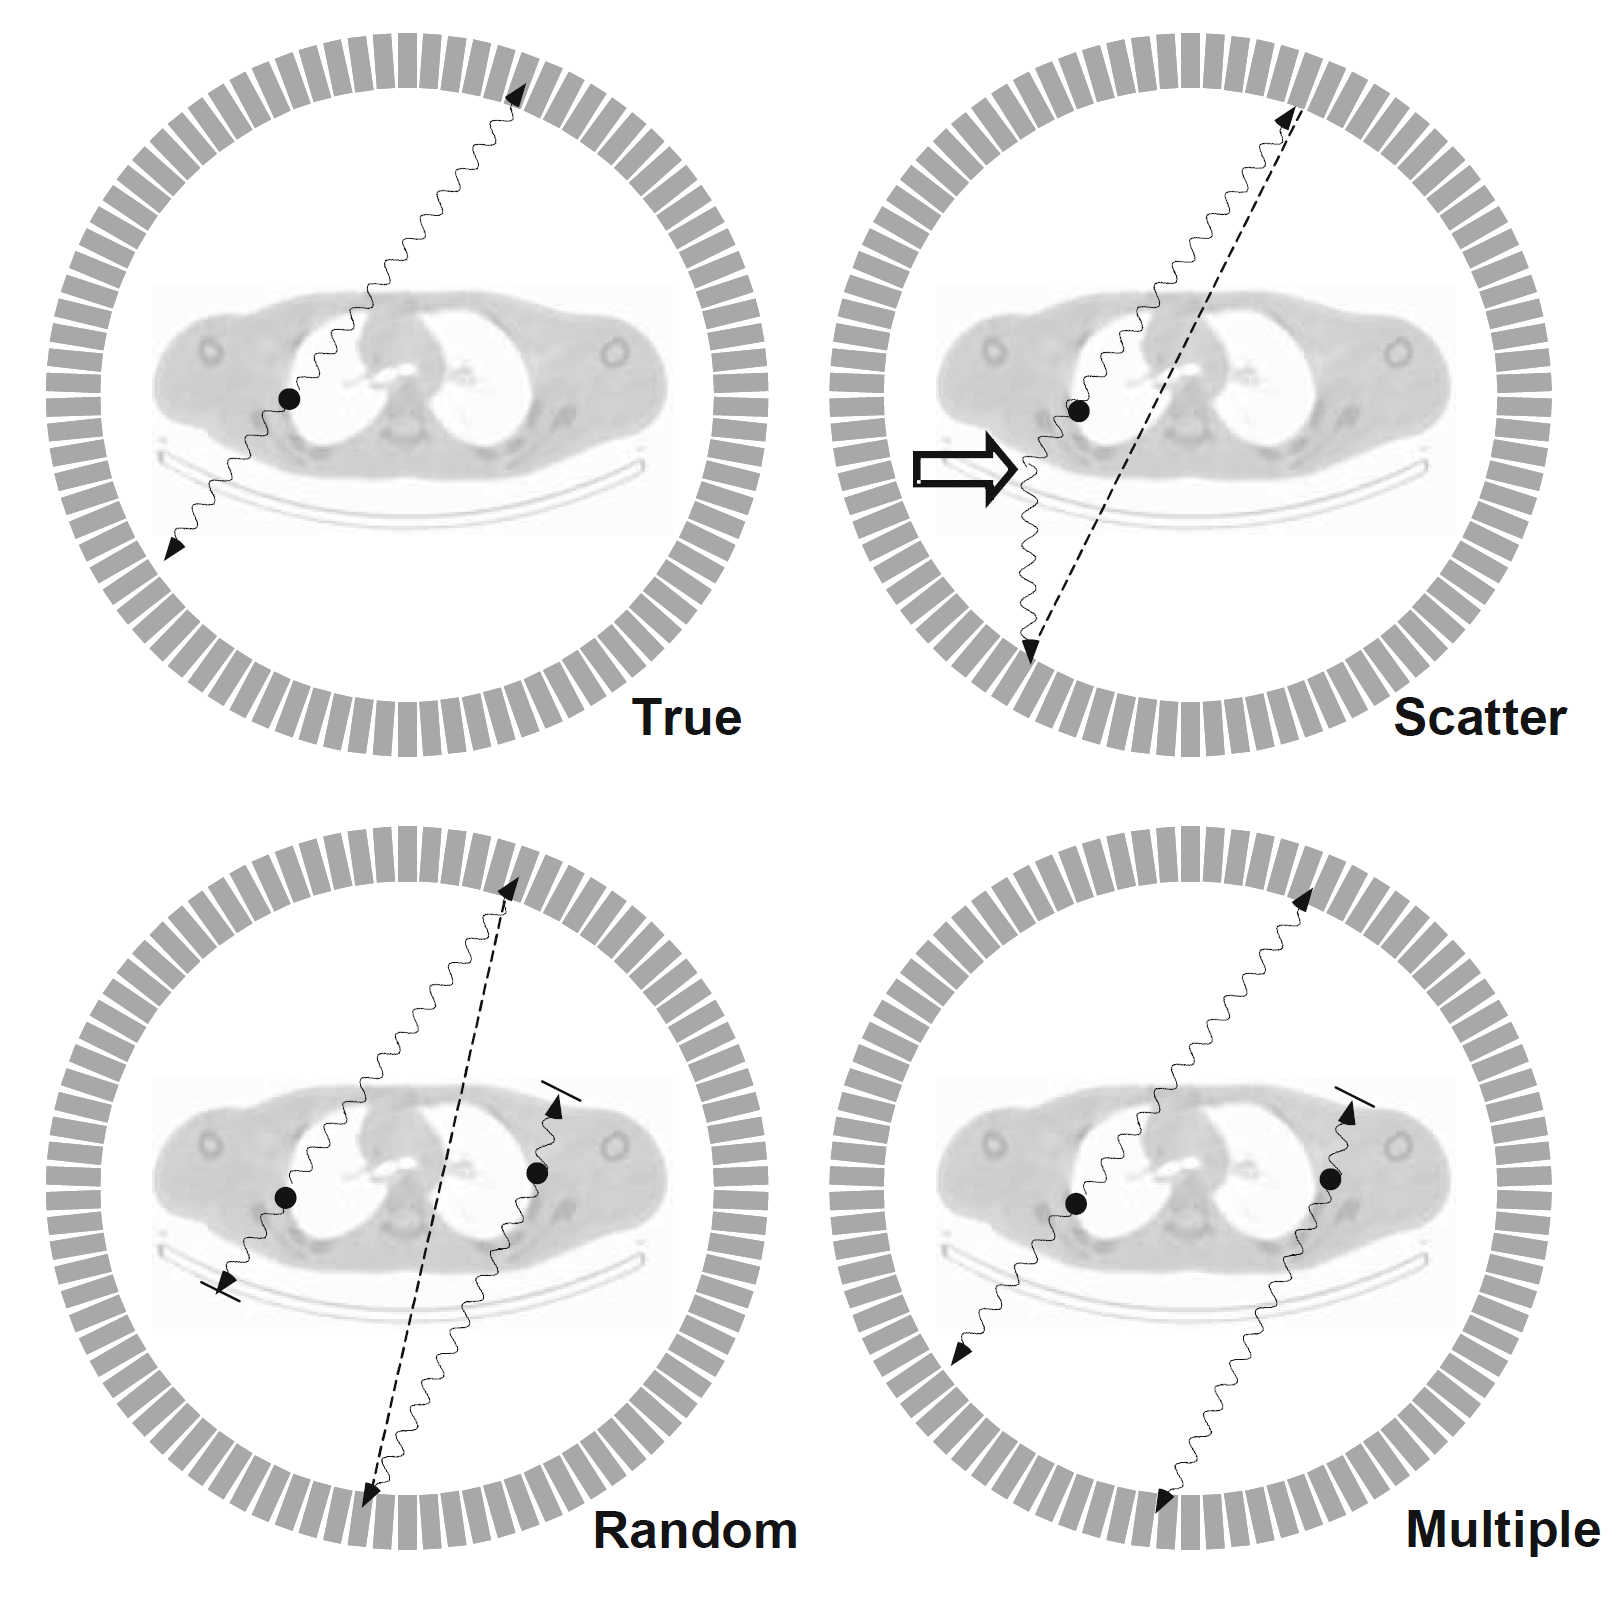
\includegraphics[scale=0.22,angle=0]{2_Theory_Methods/figures/Bailey_Scatter_Random_events.png}
\caption{Representation of different types of detected coincidence events. Adapted from Bailey~\textit{et al.}~\cite{Bailey2005}.} 
\label{fig_2:EventsIlustration}
\end{figure} 
%
%
\subsection{PET acquisition}
As described the ring formation of PET detectors is the dominant geometry used in PET systems. Using multiple rings results in the increase of \gls{afov}, solid angle coverage and possible combinations of detectors meaning a higher number of ~\glspl{lor}. But early multi ring systems were making use of 2D acquisition, where only direct and cross-plane ring coincidences were allowed. This was enforced using tungsten septa between rings, as seen in figure~\ref{fig_2:2D3D}. %The use of cross-planes allowed for the increase in axial resolution and the septa result in a uniform axial sensitivity profile as seen in figure~\ref{fig_2:2D3DSensitivityProfiles}.

With evolving detector and electronics technology, 3D acquisition became possible and is now the standard acquisition mode. 3D acquisition offers the same data as 2D acquisition and also includes all the oblique \glspl{lor} data resulting in an increase of sensitivity (4 to 6 times)~\cite{Fahey2002}. The use of oblique views leads to non-uniform sensitivity profiles in the axial direction due to the higher number of \glspl{lor} closer to the centre of the \gls{afov}, with the maximum sensitivity at the centre and a minimum at the edges of the \gls{afov}. A comparison between the 2D and 3D sensitivity profiles is shown as an example in figure~\ref{fig_2:2D3DSensitivityProfiles}.
In addition to more coincidence events, the higher sensitivity and acceptance of single events results in an increase of randoms and scatter events, which in addition may now be originating from activity outside the \gls{afov} of the system. 
%
\begin{figure} [h!]
\centering
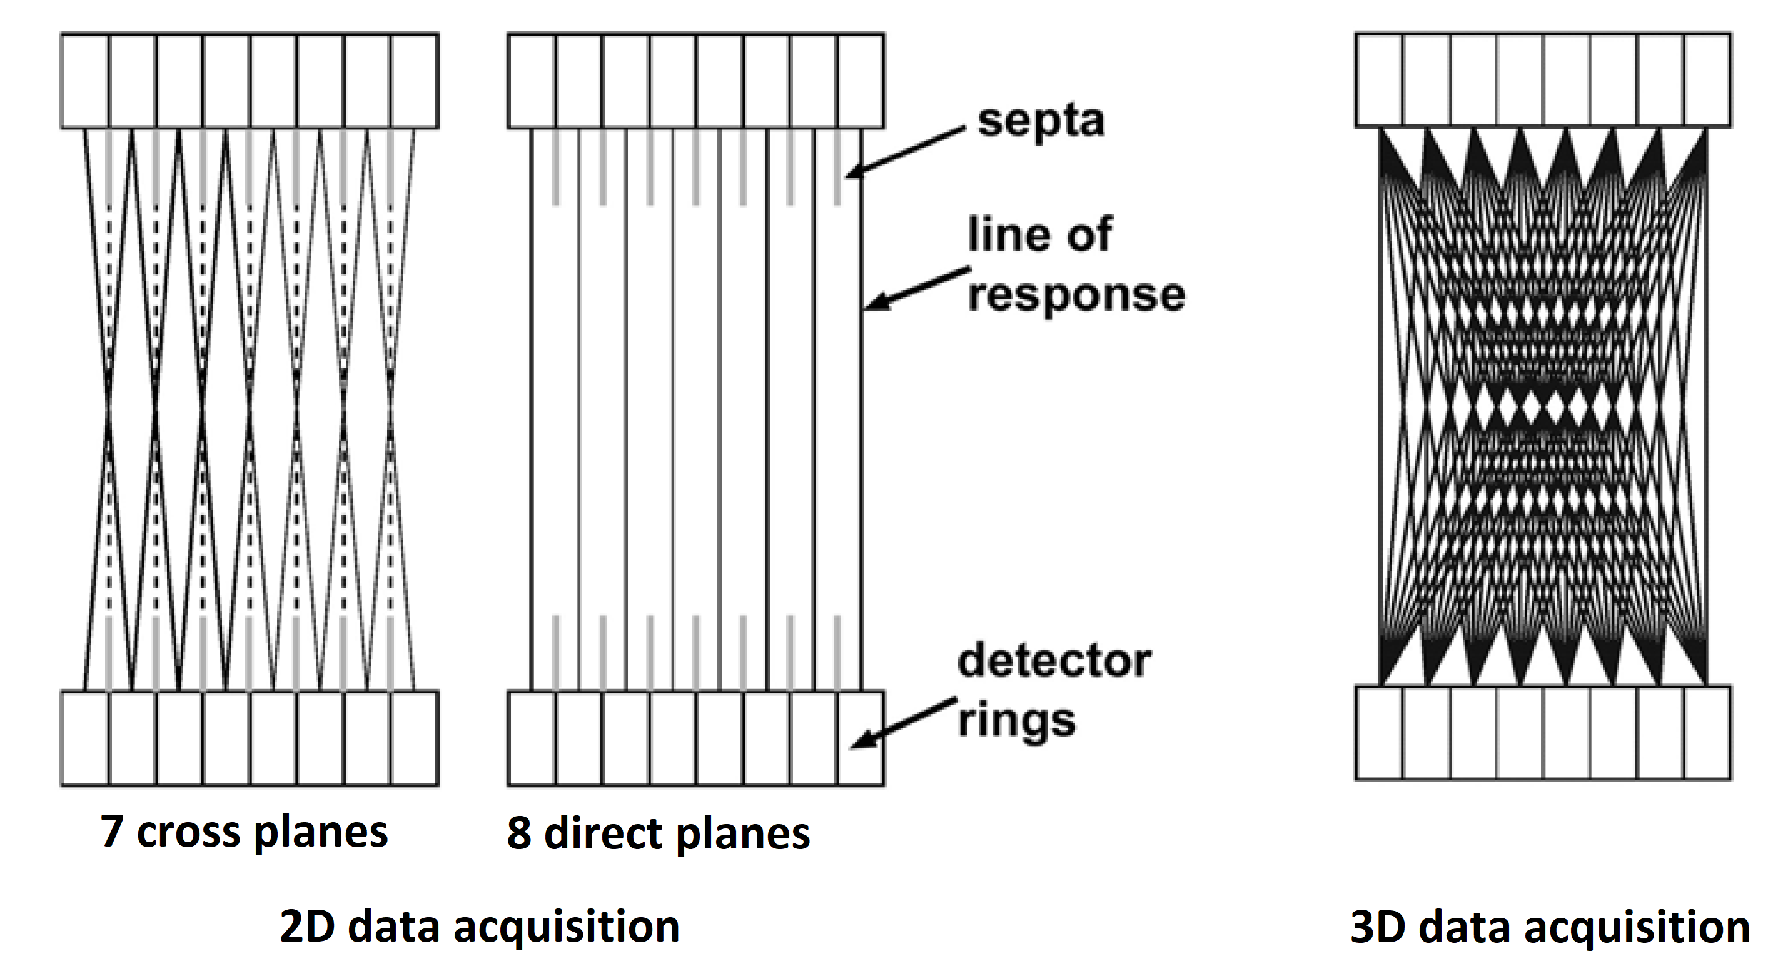
\includegraphics[scale=0.40,angle=0]{2_Theory_Methods/figures/Phelps_2D_3D_Acquisition.pdf}
\caption{Example illustration of LORs for 2D acquisition mode using direct and cross planes (left) and 3D  acquisition mode (right) for an 8 ring scanner with 15 axial slices. Adapted from Cherry S. and Magnus D.~\cite{cherry2004pet}} 
\label{fig_2:2D3D}
\end{figure} 

\begin{figure} [h!]
\centering
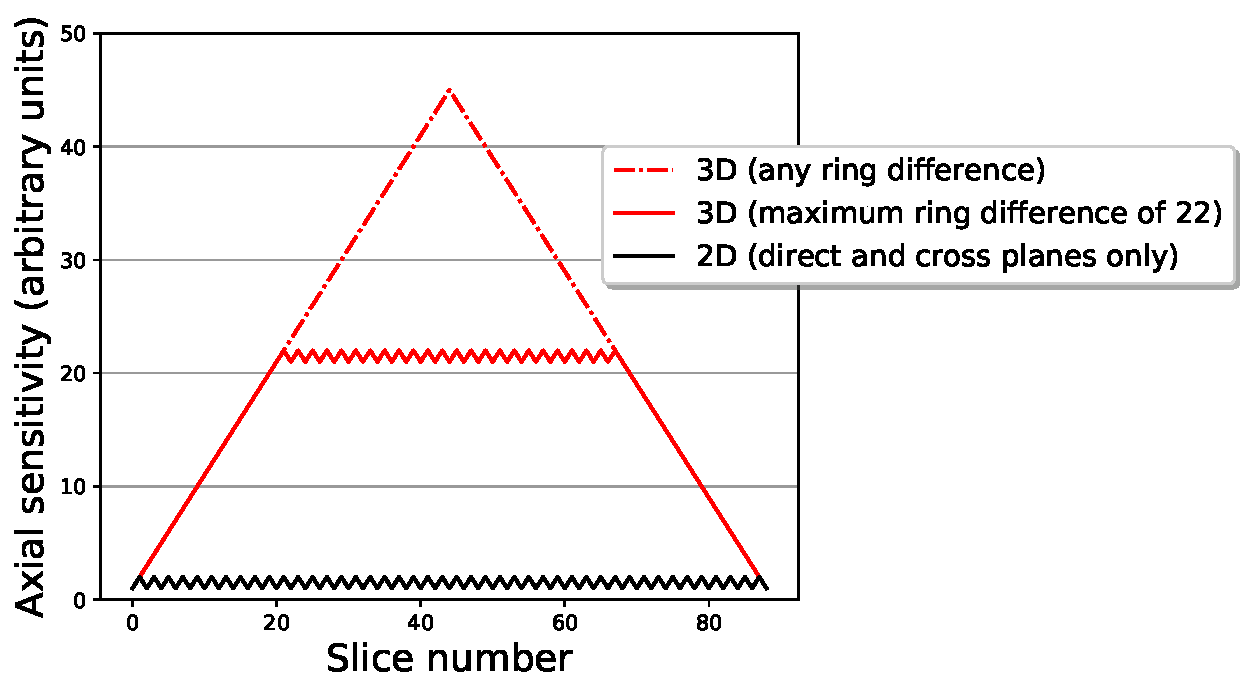
\includegraphics[scale=0.50,angle=0]{2_Theory_Methods/figures/2_2_2D3DSensitivityProfiles.pdf}
\caption{Example of 2D and 3D axial sensitivity profiles, with and without maximum ring difference limits, for a scanner with 45 direct planes which provides 45 direct and 44 cross-plane.} 
\label{fig_2:2D3DSensitivityProfiles}
\end{figure} 
%
%
In 3D mode the maximum angle of events accepted in the axial direction can sometimes be limited by enforcing a maximum ring difference permitted \glspl{lor}. This results in a uniform axial sensitivity profile at a central region of the \gls{afov}, as seen in figure~\ref{fig_2:2D3DSensitivityProfiles}.
%
%In multiple beds acquisition, used to image objects with a length larger than the scanner \gls{afov}, in order to maintain an uniform axial sensitivity a degree of overlapping is used. This allows for the regions at the edges of the bed positions to be sampled in two bed acquisitions and even out the sensitivity of the combined acquisition. The degree of overlapping can vary, depending on requirements of sensitivity uniforming and speed of acquisition.
%
\subsection{Storage of PET coincidence events}
The recorded coincidence data are stored digitally to allow post processing and reconstruction of image data.
The different methods for storing the data can result in different storage requirements, allow or not allow for specific event information to be stored and even necessitate different reconstruction techniques. 

\begin{itemize}

\item\textbf{List Mode}\\
In the simplest form coincidence events can be stored in a binary file as a stream of events by the order of their detection. This format follows naturally the detection process and allows for multiple detector information to be included in each event. A time tag is normally included in the data stream every millisecond. The minimum information recorded per event is the detector pair IDs. Any additional information such as time-of-flight, detection energy, etc. can also be included with each event. For time-of-flight the data can include exact arrival time differences, to make best use of the information in post processing or reconstruction methods.
The use of list-mode files is practical for dynamic studies as they naturally include all dynamic information and can take less storage space than the other alternative formats described below. List-mode data can be binned into the formats described below before reconstruction or used directly with list-mode reconstruction algorithms. 

\item\textbf{Histogram}\\
Coincidence events per detector pair (\gls{lor}) can be summed together and stored into a single entry. The total number of entries will be equal to the total number of detector pairs. These entries make up a histogram, where effectively all the events have been histogrammed into the detector pairs. No timing information is preserved and hence multiple histograms are required if data are recorded dynamically, in a predefined temporal binning. 
This format can result in smaller files for static imaging compared to list-mode, but in the case of dynamic imaging it frequently results in a much larger total size of files as multiple detector pair entries are empty (zero) for some time frames. Furthermore, if time-of-flight information is also available, separate histograms need to be created for each time-of-flight bin (discretization of the TOF resolution), which further increases the zero entries and storage requirements. 
Compression is possible in both axial and transaxial direction of the data, which is referred to as axial compression (or span) and angular compression (or mashing) respectively~\cite{Fahey2002}. These are employed by some scanner manufacturers to counteract the increasing size of histograms from increasing scanner resolution and better TOF resolution. The compression strength is chosen as a trade-off of file size and degrading image quality properties~\cite{Belzunce2017}. 

\item\textbf{Sinogram}\\
Sinograms are representations of the data in projections through the process of projection using a transformation such as the Radon or X-Ray transform~\cite{Natterer1986}. Each pixel of the sinogram represents the integral of events over a specific line through the image space. The name "sinogram" comes from the fact that a point source (off-centred) is represented as a sine wave in the sinogram.
The use of sinograms is inherited from other tomographic imaging methods where data are acquired as projections. Sinograms are used with analytical reconstruction methods, shortly described in chapter~\ref{Chap2_3:Reconstruction}, which require the projection space to be fully and uniformly sampled.
%In \gls{pet}, contrary to list-mode and histograms where the data are directly related to detector elements, conversion of data to sinograms requires certain processing steps to ensure 
%As seen in figure~\ref{fig_2:Sinogram_detector_to_Sino}, parallel \glspl{lor} at a specific direction are used to form the sinogram along a particular row. The sampling of the sinogram space will depend on the size of the sinograms required, and data conversions will be required  to match the required sinogram sampling \cite{Fahey2002}. 
%
%\begin{figure} [h!]
%\centering
%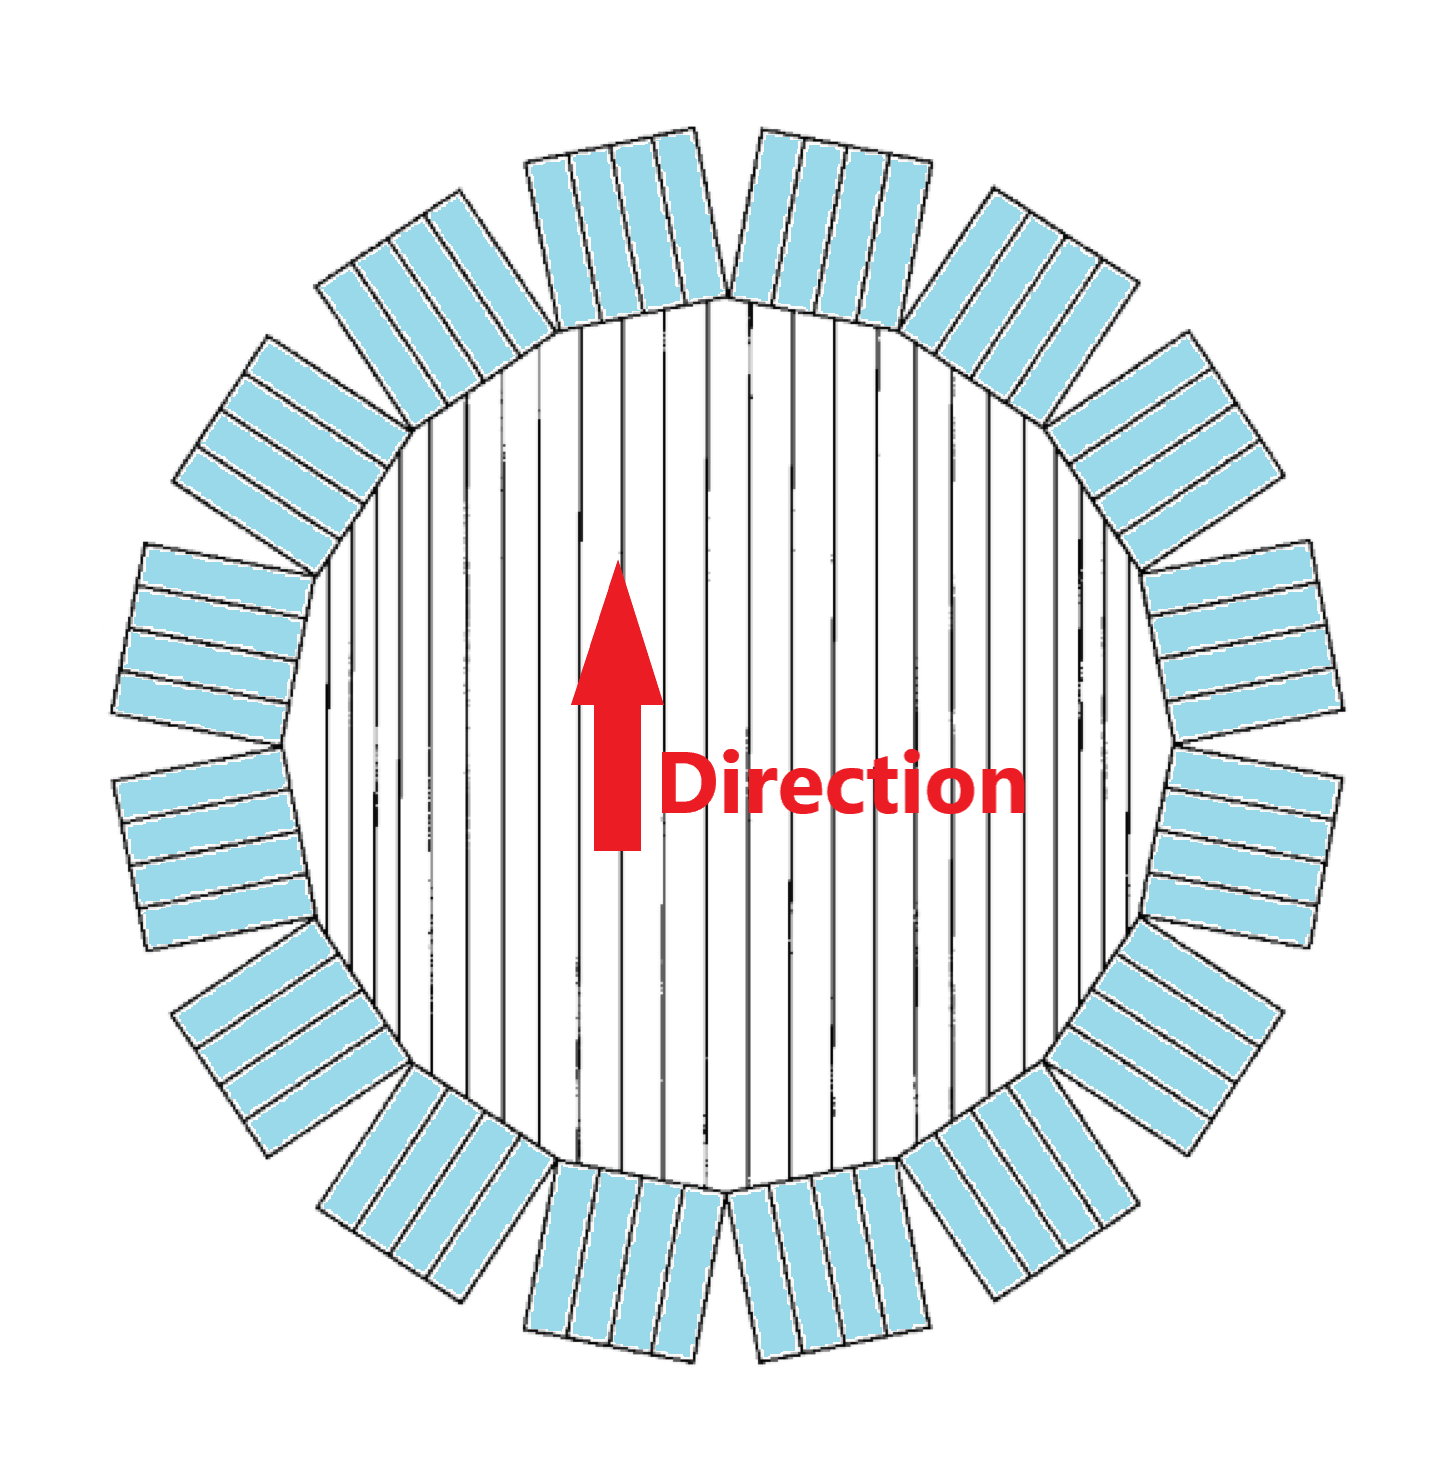
\includegraphics[scale=0.15,angle=0]{2_Theory_Methods/figures/Sinogram_detector_to_Sino.png}
%\caption{Example projection though the PET field of view for a specific direction~\cite{Fahey2002}.} 
%\label{fig_2:Sinogram_detector_to_Sino}
%\end{figure} 
%
%In practice events can be detected in any angle within the transaxial plane as well as the axial planes that are defined by the multiple detector rings that form the \gls{pet} system. In 3D acquisition, crystals from all rings (or under certain maximum ring difference limitations) are allowed to record coincidences. In this case the number of sinograms increases to allow all the possible co-planar angle combinations, and the radon transform is extended in 3D. With the introduction of time-of-flight information, a separate set of sinograms is required for each TOF bin and when dynamic data are captured a separate set per temporal bin. In practice different types of compression have been used to reduce the total size of sinogram raw data.
\end{itemize}

As in this project we did not make use of analytical reconstruction algorithms, we have not described the formation and use of sinograms in detail. 
In the project, we made use of both real data from clinical PET scanners and simulated data from analytical simulations. For real data we made use of the list-mode data format, to reduce file size and allow for flexibility in the treatment of the data, while for simulations we used the histogram data format as we were limited to that by the nature of analytical simulations.
It is important to note that clinical PET systems are performing reconstructions using histograms or sinograms and although they can record data in list-mode format, they always re-bin the data to histograms or sinograms before performing a reconstruction. 
By contrast in this project, we made use of list-mode reconstruction algorithms when using list-mode datasets.

\subsection{PET Corrections and Quantification}
PET has always been used as a quantitative imaging method, providing image values that relate to radioactivity concentration. This is an important requirement for semi-quantitative and quantitative interpretations of the imaged data, with quantitative measures being at the foreground on this thesis project.
But accurate quantification of images requires corrections that need to be considered before and during the reconstruction process. The main corrections needed for quantifiable PET are outlined here.

\begin{itemize}
\item\textbf{Randoms correction}\\
As discussed previously, random events in the data are estimated using delayed coincidence detection or by measurements of single event rates between detectors. For most clinical scanner manufacturers and for list-mode data these are normally provided in the same stream of data, with delay events recorded similarly to prompts and with single events recorded for every predefined time interval (for example every second) for each detector or detector block. Similarly, for histogram data, a separate histogram of random events is provided. A histogram per frame (time bin) is required for multiple frame datasets, for randoms as well as for prompt events. 
In the reconstruction software used in this projects, \gls{castor}~\cite{Merlin2018}, the corrections are provided for each event \gls{lor} or histogram within the raw dataset file. Furthermore, randoms corrections in \gls{castor} are provided in rates (s$^{-1}$) which is a more natural format to use with list-mode data reconstruction and dynamic datasets.
\item\textbf{Scatter correction}\\
As described previously, a certain amount of the annihilation gammas will scatter with the atoms of the travelling medium via Compton scattering, which results in changes of energy and direction of the gammas. Even after the energy filtering applied on the detectors, an amount of those scattered gammas will be detected and recorded as coincidence events that degrade the PET data and affect image quality and quantification. The most commonly used approach to account for scatter in clinical scanners is the use of the Single Scatter Simulation algorithm~\cite{Watson1996} to estimate scatter. These simulations are based on an initial activity distribution estimate from the uncorrected PET data and knowledge of the probability of scattering. 
Scatter estimates, similar to random estimates, are then used as additive corrections within statistical reconstruction methods. Again, in~\gls{castor} these are provided as \mbox{rates (s$^{-1}$)}. 
\item\textbf{Normalisation}\\ 
Sensitivity between \glspl{lor} will differ due to detector and geometric efficiencies effects. Normalisation coefficients for each \gls{lor} are estimated using measurements and modelling of the normalisation components and are subsequently used in reconstruction to correct for these efficiencies.
\item\textbf{Dead-time correction}\\
After every detection event, a certain amount of time is required for sub-systems involved in the detection to become ready for detection again and so interaction events occurring during that recovery time will not be registered. As the number of interactions increases at higher imaged activities, the proportion of events not registered is also increasing. The result is a non-linear system response for different levels of imaged activities. This effect is corrected using dead-time correction which is applied by the of lookup tables that relate single rates to dead-time factors and real-time singles monitoring measurements.
\item\textbf{Attenuation correction}\\
Absorption or scatter interactions within the body results in loss of gammas detection. Even if one of the two annihilation gammas is lost the result is a non registered event. The probability of attenuation depends on the total probability of interaction within a \gls{lor} and is independent of the annihilation position within that line. This enables the estimation of attenuation factors for each \gls{lor} within the body by use of transmission measurements, either with radioactive sources or X-rays sources. For these measurements earlier scanners made use of positron or single gamma sources to estimate attenuation while most modern clinical systems make use of \gls{ct} or \gls{mr} scans to estimate attenuation factors. 
\item\textbf{Calibration Factor}\\
%Contrary to other nuclear medicine techniques, \gls{pet} is fully quantitative and can be used to deduce absolute activity measurements from the reconstructed image data. 
Finally, after all other corrections have been applied there is a need for a global calibration factor to relate the estimated number of true events to activity concentration. 
PET systems are calibrated against a reference source to obtain such factors. 
\item\textbf{Decay correction}\\
Finally, measurements need to be corrected for decay of the imaged radionuclide for the duration of the acquisition and for decay-correction to a reference time. 
For static imaging, the reference time is chosen to be the imaging start time, while for dynamic acquisitions the reference time is commonly chosen to be the time or tracer injection. 
\end{itemize}

\section{Hybrid PET Systems}
\subsection{PET-CT}
As described above attenuation correction is essential for quantitative \gls{pet} imaging. Early \gls{pet} systems made use of external radioactive sources to acquire a transmission scan. Some of the drawbacks of these methods were that transmission scans would contribute to an increase of image noise on PET images and that transmission scan acquisition was increasing the total duration of the examination.
As PET imaging became more frequently used in clinical applications, the need for fusion of PET images with CT images became apparent, firstly for the clinical value by complementary PET functional images to CT anatomical images and secondly for aiding in attenuation correction and anatomical localisation. These needs led to the development of the first hybrid PET systems, with the first PET/CT system being introduced in the late 1990s~\cite{Townsend2008}.
The first PET/CT was able to acquire a whole body PET/CT scan, using multiple bed positions as it will be described later in this chapter, within an hour with precisely co-registered CT and PET images that were acquired close in time~\cite{Beyer2000}. The CT scan was used in PET attenuation correction via scaling of attenuation factors to account for the energy difference between CT and annihilation photons~\cite{Kinahan1998}. PET/CT eliminated the need for radioactive source transmission scans and the problems with excessive noise associated with these relatively poor quality transmission images.

\subsection{PET-MR}
\label{sec:PET_MR_Systems}
MRI provides anatomical images with higher soft-tissue contrast than CT imaging. The option of different acquisitions sequences can allow for different types of soft-tissue contrast, which can also extend to dynamic and parametric MR imaging applications~\cite{Besson2020} and also to functional MRI~\cite{Kolb2012}.
The fusion of PET and MR was technically challenging due to interference between the two systems~\cite{Disselhorst2014}.
Initial PET and MR clinical workflows and systems made use of separate PET and MR or PET/CT and MR scanners to scan the patient using a single bed to transfer the patient from one scanner to the other and minimise patient misalignment~\cite{Zaidi2011,Veit-Haibach2013}.

The use of PMT based detectors for synchronous PET/MR imaging was only possible using long optical fibres that shifted the detection of events by the PMTs at a safe distance away from the centre of the magnetic field~\cite{Shao1997,Mackewn2010}. Later advancements in PET detector technology allowed for Avalanche photodiodes (APD) and silicon photomultipliers (SiPM) based detectors, which led to the development of PET inserts~\cite{Kolb2012} for MR and the development of fully integrated PET-MR systems that perform synchronous acquisitions~\cite{Delso2011,Grant2016,Levin2016}.
There are currently two PET/MR integrated systems by commercial manufacturers, the Siemens mMR and the GE Signa. In this project, we relied on access and real PET data from a GE Signa PET/MR that is available in our centre. But we also made use of Siemens mMR data in a collaboration project with the Medical University of Vienna that is described in the Secondary Contributions section at the end of this manuscript. 

The Signa PET/MR scanner was designed based on an existing 3 Tesla MR scanner (3T MR750w MR scanner) that was modified to accommodate the PET detector ring. The ring comprises of 28 modules with 720 scintillator crystals per module. Those were coupled with SiPM detector modules, which are capable of capturing TOF information. A schematic of the modules and their integration in the system ring is shown in figure~\ref{fig_2:SignaPETMR_Integrated_System}. The PET ring provides a total of 89 slices and an \gls{afov} coverage of approximately 25 cm with a slice thickness of 2.78 mm.

\begin{figure} [h!]
\centering
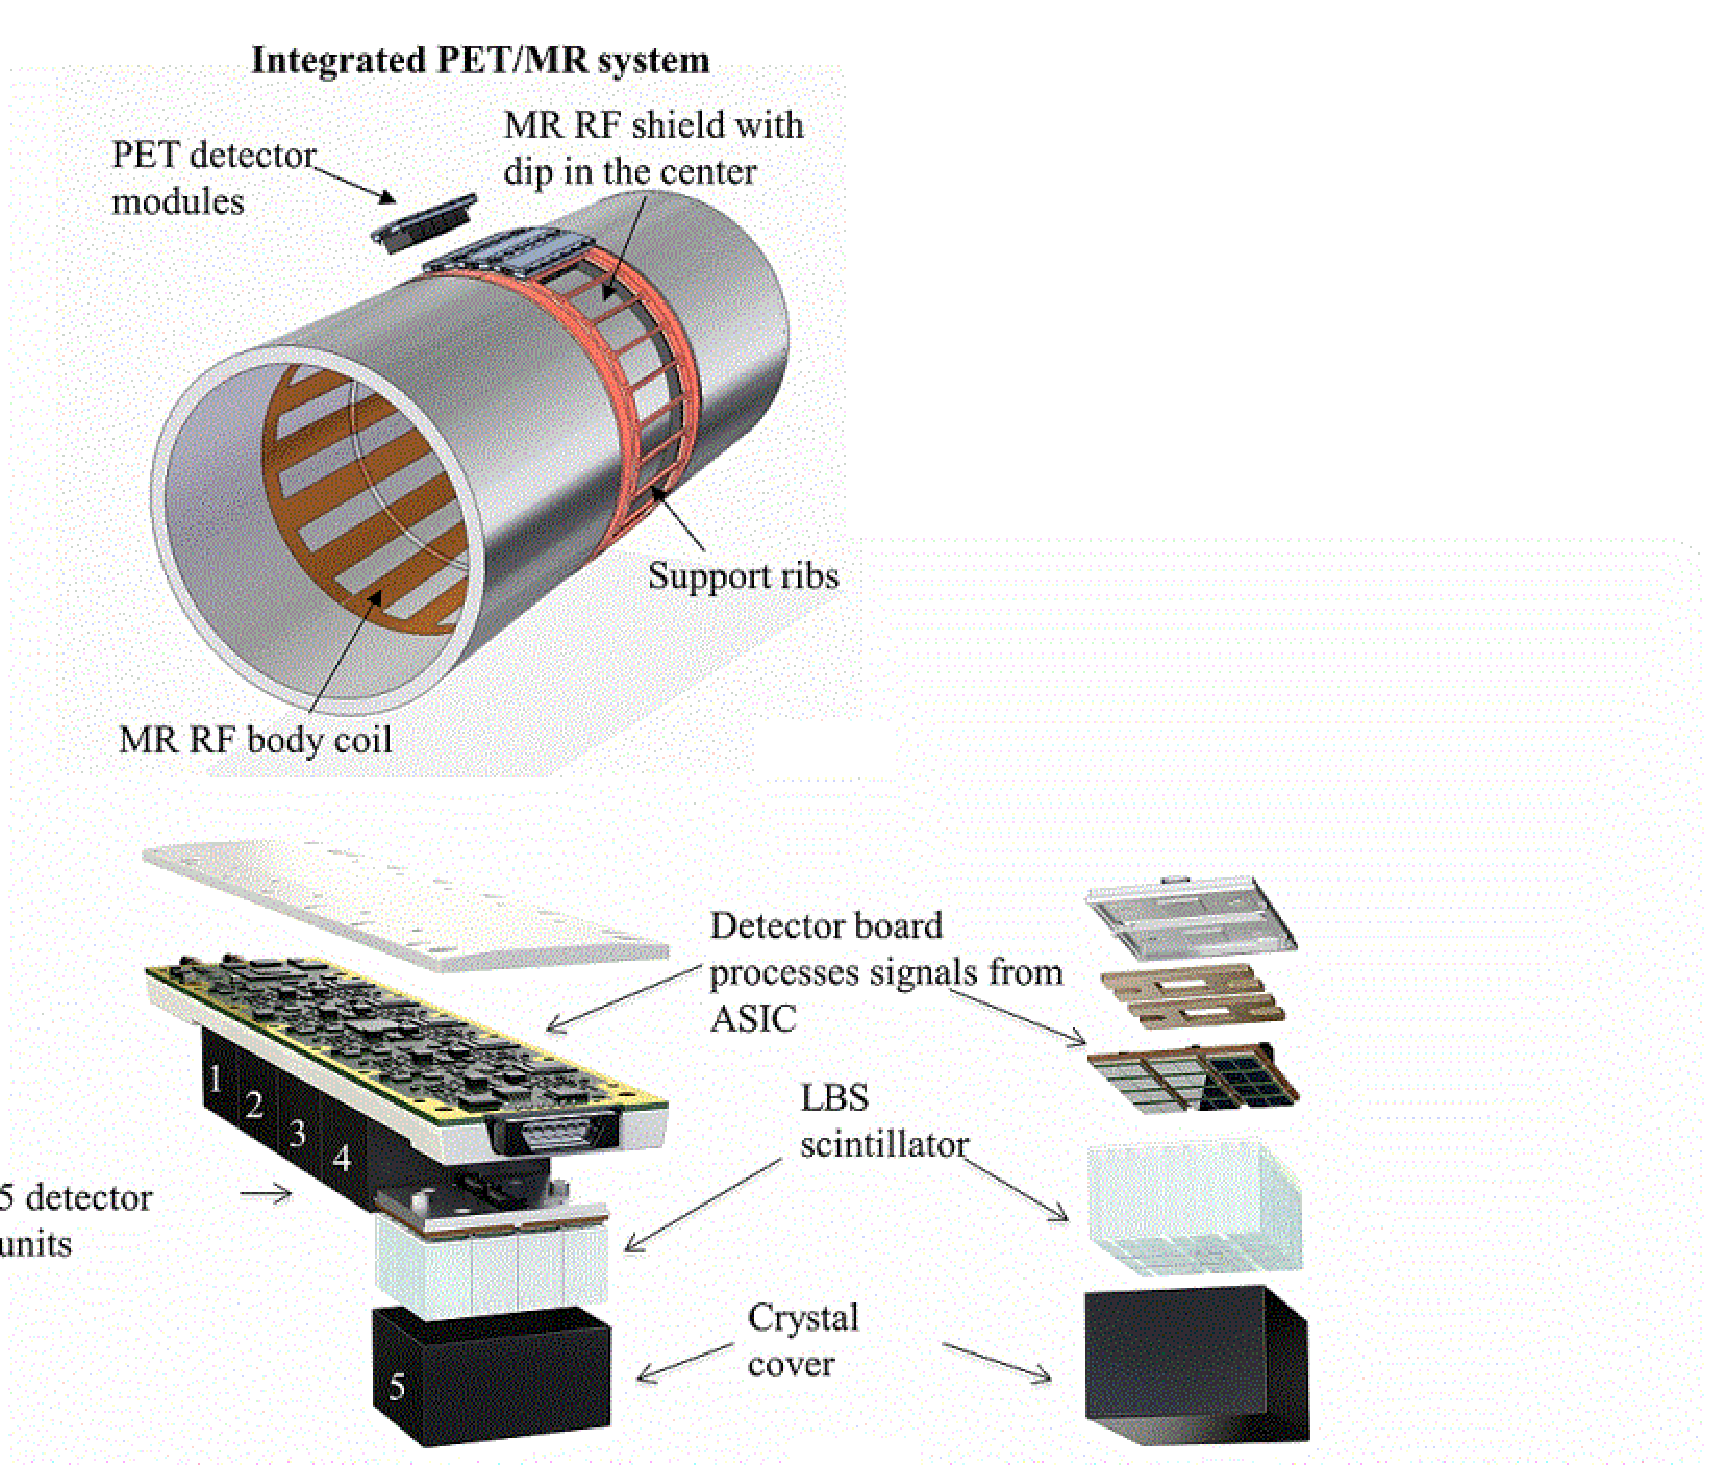
\includegraphics[scale=0.45,angle=0]{2_Theory_Methods/figures/SignaPETMR_Integrated_System.pdf}
\caption{Schematic of the GE Signa hybrid PET-MR system, comprising of detector module units (bottom) in a ring formation within the MR RF body coil (top)~\cite{Levin2016}.} 
\label{fig_2:SignaPETMR_Integrated_System}
\end{figure} 

\section{Whole Body PET: Static Imaging}
For many clinical applications, as for example in oncology, PET imaging over the whole body is essential for the detection and characterisation of primary and metastatic disease. Developments in PET detectors technology and reduction of production costs have resulted in increasing axial length of PET scanners using additional detector rings, with currently widespread clinical models offering between 15 to 26 cm of axial coverage~\cite{Vandenberghe2020}.
In practice for static imaging whole-body coverage is achieved using multiple bed positions. The first suggestion and optimization work in extending the effective A-FOV of PET scans using multiple bed positions was made by Dahlbom~\textit{et al.}~\cite{Dahlbom1992}. This work was made on PET systems operated in 2D mode, where a bed displacement of approximately equal to the system's A-FOV was used to increase the acquisition's effective A-FOV. As systems became capable of acquiring in 3D mode, offering increased sensitivity but resulting in axial varying sensitivity profiles, different strategies were needed for multi-bed acquisitions. The two methods suggested and developed are the \textit{Step and Shoot} (SS)~\cite{Schubert1996} and the \textit{Continuous Bed Motion} (CBM)~\cite{Panin2014} acquisition methods.

\subsection{Step and Shoot}
\label{WB_Static_SS}
The SS method makes use of multiple bed positions that are partially overlapped in the axial direction to increase the sensitivity of the acquisition at the edges of adjacent beds, by combining data of adjacent beds over the overlapping region as shown in figure~\ref{fig3_1:fullOverlap}. 
One way of combining the multi-bed datasets is to reconstruct each bed individually, displace the reconstructed images according to their axial location and combine them using weighted averaging~\cite{Schubert1996}. This method has prevailed in clinical PET systems that use the SS acquisition method, as it does not require additional considerations in the reconstruction process of each bed and the combination of bed images can be performed post-reconstruction. Alternatively, the axial displacement of each bed raw dataset can be performed during the projection and back-projection process in iterative reconstruction, which then directly results in the reconstruction of the whole-body image~\cite{Ross2004}. Use of the overlap data in iterative reconstruction can potentially result in improved noise characteristics at the overlapping regions, as the full sampled statistics over these regions are combined prior to each image update~\cite{Ross2004,Stute2014}. 
%
\begin{figure} [ht!]
\centering
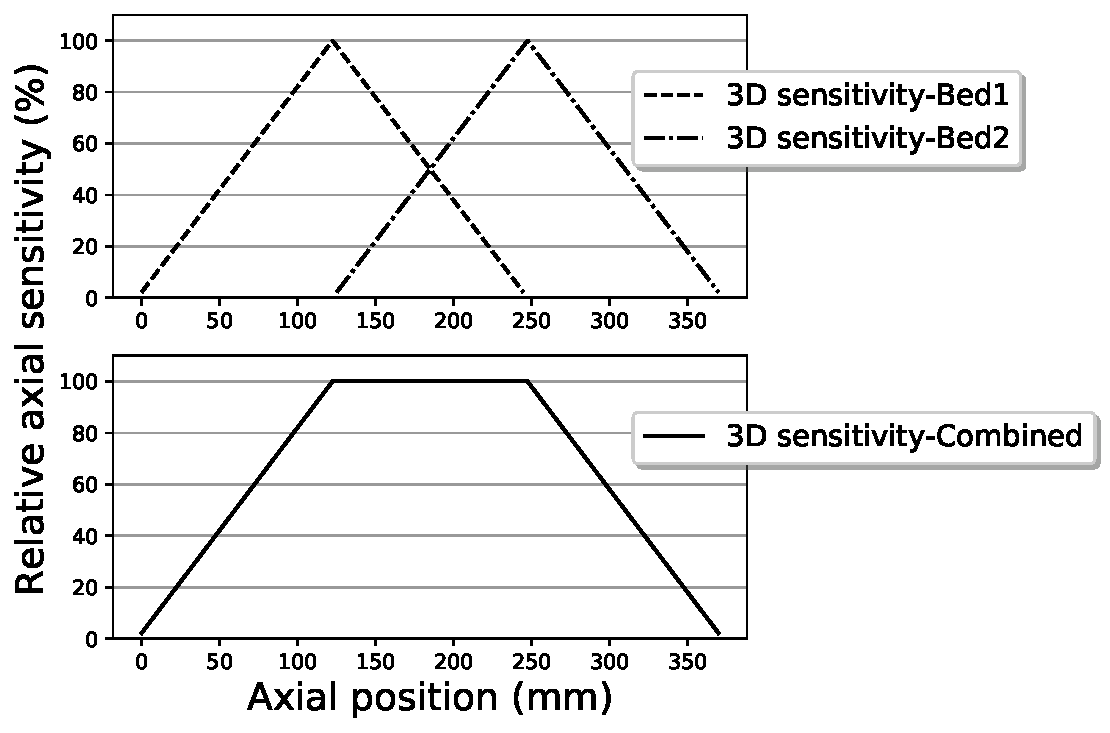
\includegraphics[scale=0.6,angle=0]{2_Theory_Methods/figures/SensitivityProfiles_fullOverlap.pdf}
\caption{Relative axial sensitivity of individual beds (top) and combined sensitivity profile (bottom) for approximately 50\% overlap for the Signa PET/MR.}
\label{fig3_1:fullOverlap}
\end{figure}
%
%The amount of overlap is a parameter to select according to the needs of the axial sensitivity profile.
The axial sensitivity profile for the Signa PET-MR system is shown in figure~\ref{fig3_1:fullOverlap}, where to result in a completely uniform axial sensitivity profile an overlap of 44 slices ($\sim$50\% of \gls{afov}) is required.
The amount of overlap used depends on the needs for uniformity in axial sensitivity and reconstructed image noise. This in term will also depend on the used reconstruction type and the activity distribution of the imaged subject~\cite{Schubert1996}. 
For standard clinical scanning at the Signa PET-MR an overlap of $\sim$27\% is used by default, to balance between sensitivity uniformity and examination time for standard WB examinations. The trade-off is made between the effective A-FOV and the total acquisition time, with the latest being of practical importance for patient comfort and high throughput. In addition, the acquisition time per bed is also an important parameter that affects this trade-off. For example, newer and higher sensitivity scanners can enable shorter scanning per bed for the same image quality, which allows for increased overlapping and improved axial sensitivity uniformity at the same total scan time.
Examples of three overlapping options and the provided coverage for the Signa PET/MR are shown in figure~\ref{fig3_1:decreasingOverlap} and~\ref{fig3_1:BodyCoverage} figure respectively.
Many clinical WB protocols actually require imaging of approximately half the length of the body, from head to thighs, which can be accommodated with 5 or 6 bed positions on the Signa PET/MR. When full body coverage is required the number of beds is increased to 9 or 10. %In DWB acquisitions where fast scanning is crucial the overlap can be decreased to maintain the same coverage with a lesser number of bed positions, as shown in option(C) of figure~\ref{fig3_1:BodyCoverage}. 
%
\begin{figure} [ht!]
\centering
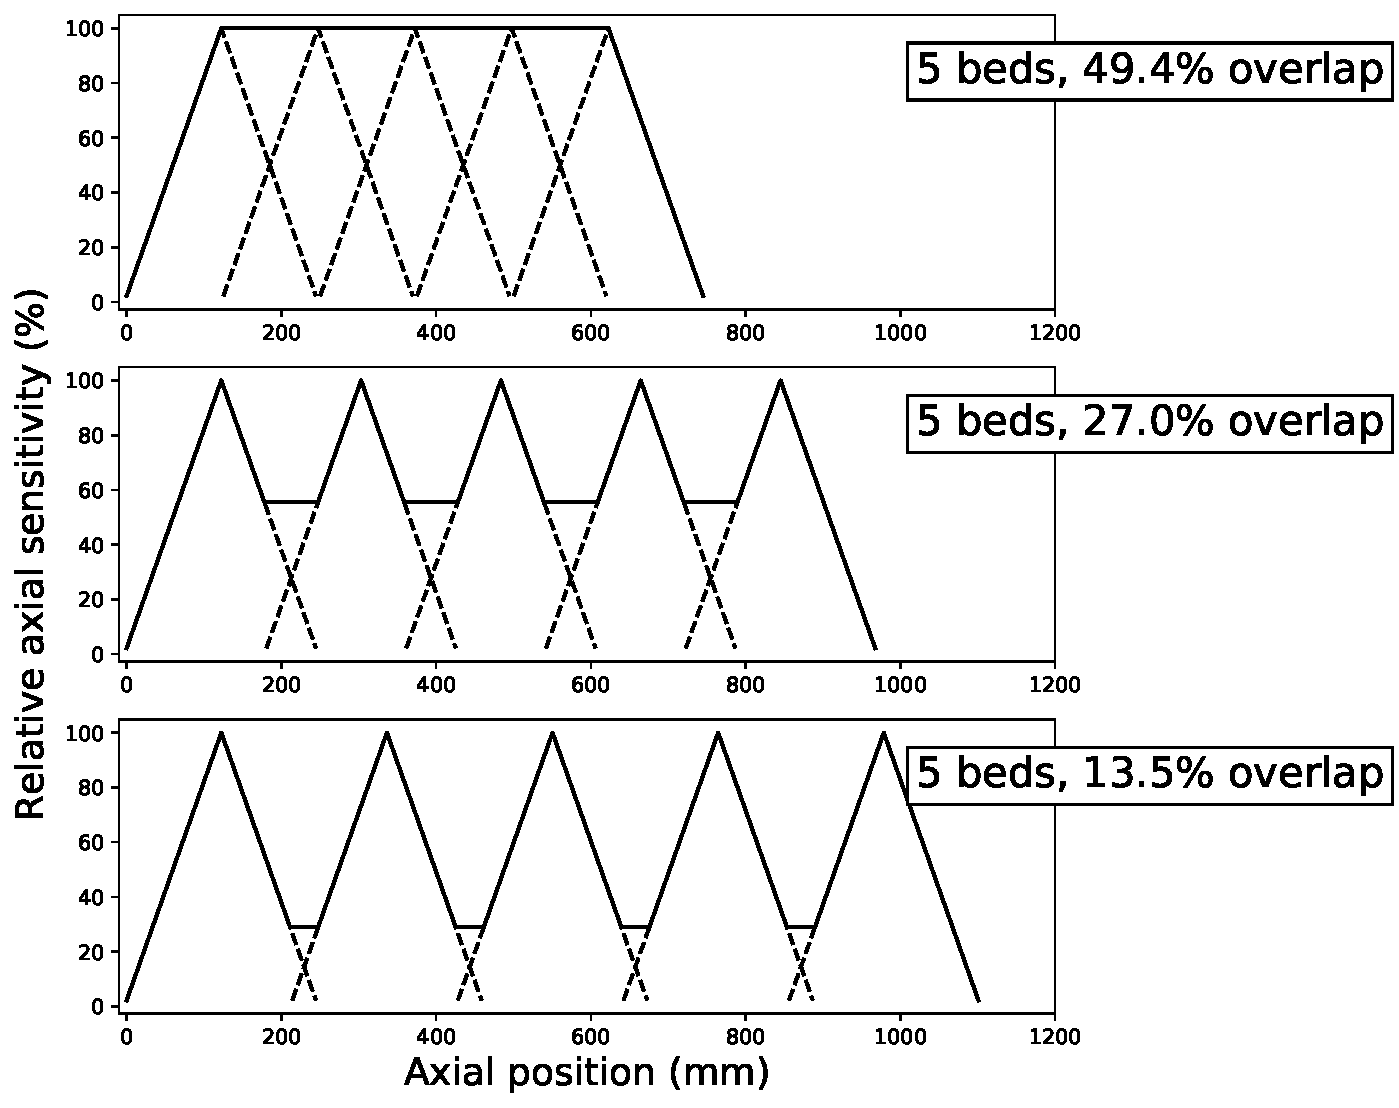
\includegraphics[scale=0.5,angle=0]{2_Theory_Methods/figures/SensitivityProfiles_3Options.pdf}
\caption{Relative axial sensitivity of 5 bed positions with decreasing overlap for the Signa PET/MR.} 
%TODO: Add over-scan in the CBM D-WB protocols. 
\label{fig3_1:decreasingOverlap}
\end{figure}
%
%
\begin{figure} [ht!]
\centering
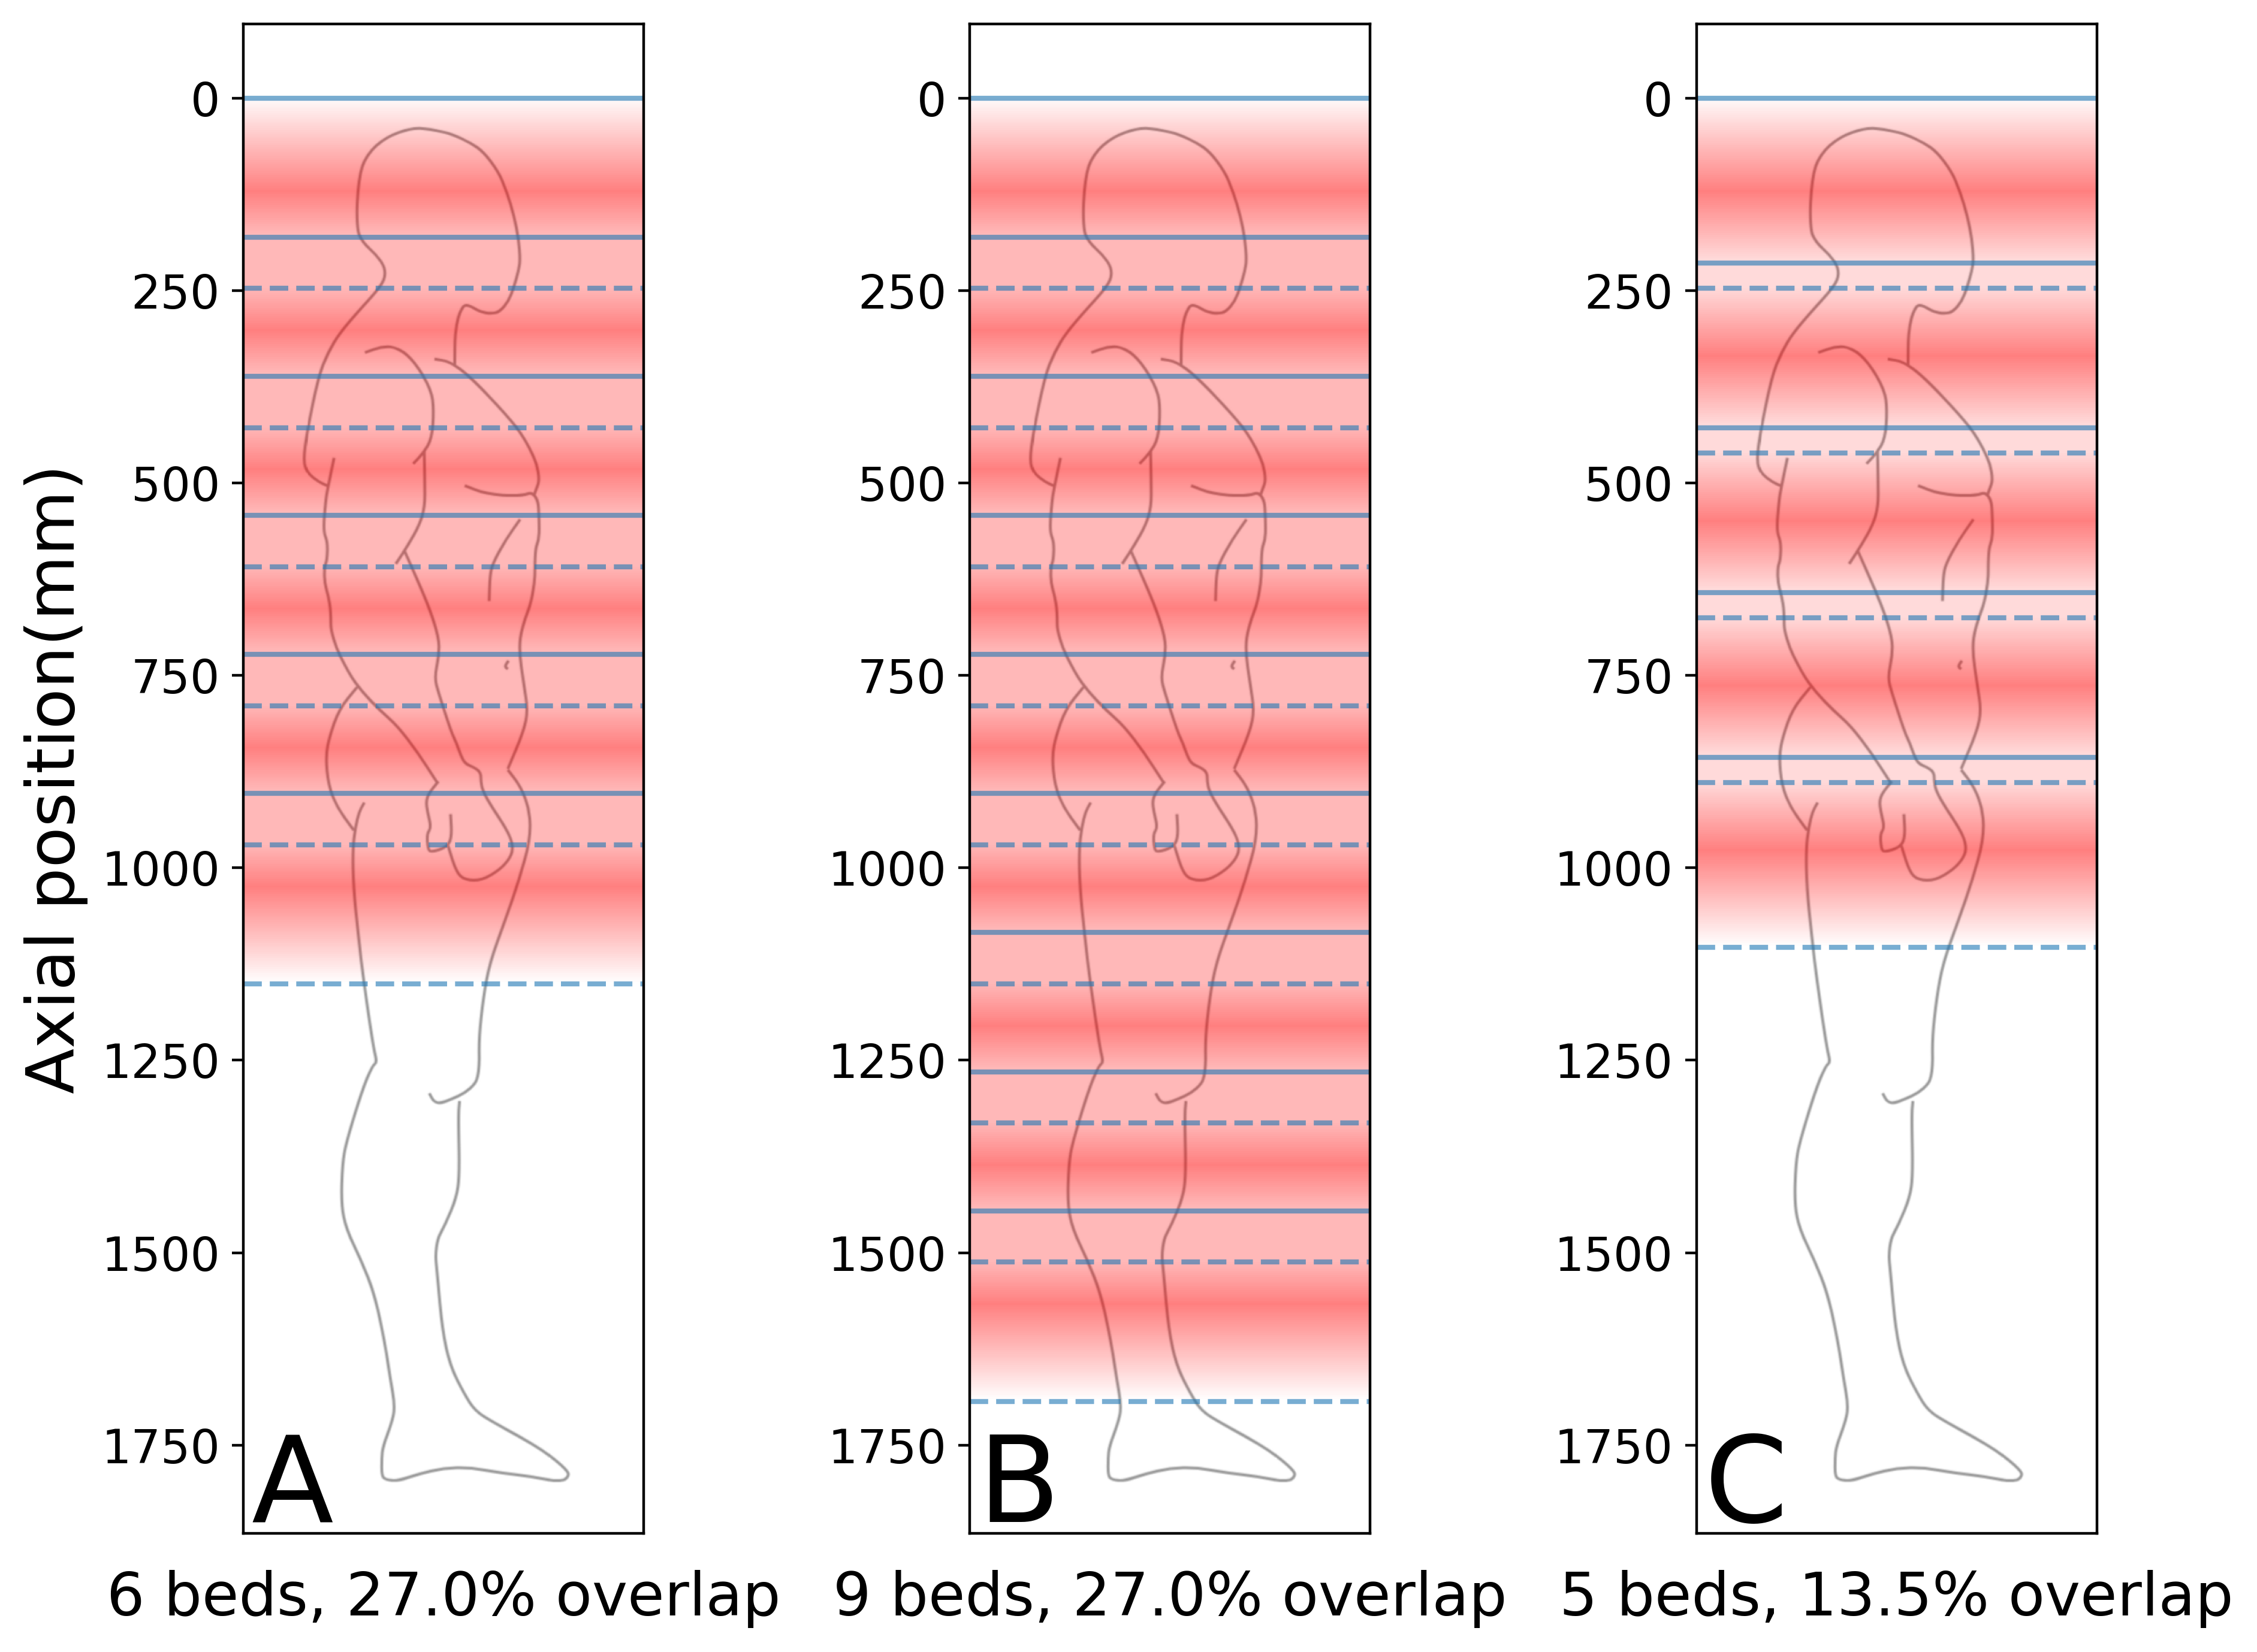
\includegraphics[scale=0.5,angle=0]{3_Results/3_1_DWB_Optimization/figures/SensitivityProfiles_overHuman.png}
\caption{Combinations of overlap and number of beds for static (A\&B) and dynamic whole-body imaging(C). Relative axial sensitivity is shown in shades of red, with bed start (\protect\tikz[baseline]{\protect\draw[line width=0.5mm] (0,.8ex)--++(1,0) ;}) and end (\protect\tikz[baseline]{\protect\draw[line width=0.5mm,densely dashed] (0,.8ex)--++(1,0) ;}) positions.} 
%TODO: Add over-scan in the CBM D-WB protocols. 
\label{fig3_1:BodyCoverage}
\end{figure}
%
%
%
\subsection{Continuous Bed Motion}
Continuous Bed Motion was proposed as an extension of step and shoot acquisition performed with small steps, to provide uniform axial sensitivity profiles~\cite{Dahlbom2001,Brasse2002}. In clinical CBM acquisition protocols, the bed positional information is stored in list-mode during the examination and the data are sorted after or during the examination in histograms or sinograms (referred as "chuncks") before reconstruction. The velocity of the bed movement can be adjusted depending on the amount of desired collected statistics, similar to the acquisition time per bed in SS acquisitions. In recent systems, the bed velocity can also be varied within an examination according to the needs and distribution of the imaged activity~\cite{Panin2014}. Beyond the potential technical gains, CBM protocols have also been shown to aid in patient comfort during examination~\cite{Schatka2016}. 
%In particular for dynamic whole-body imaging many aspects of CBM acquisition can be beneficial over SS imaging~\cite{Karakatsanis2016a}.  
%
\section{Whole Body PET: Dynamic Imaging}
As outlined in the introduction, clinical and research applications can benefit from dynamic whole-body (DWB) PET information. In clinical applications, DWB data can be used to construct fully quantitative parametric images for diagnosis and response monitoring of disease and pathology over the whole body. In research, DWB information can enable studying of the whole body organism and interactions between different tissues, organs or compartments. 

Although recent advancements in PET have led to the development of PET/CT systems with increased A-FOV, with approximately half~\cite{Karp2020,Siegel2020} or even total-body axial coverage~\cite{Cherry2018}, the majority of clinical PET systems in use are limited in the range from 15 to 26 cm~\cite{Vandenberghe2020}. 
Based on the same principles and methods used in static WB PET imaging, DWB protocols have been developed with the use of repeating whole-body passes (often referred to as "sweeps"). 
These protocols can be implemented using SS acquisition, as proposed in the original work on multi-bed DWB protocols by Karakatsanis~\textit{et al.}~\cite{Karakatsanis2011,Karakatsanis2013}, or as later proposed using CBM~\cite{Karakatsanis2016a,Hu2020}. Such protocols are nowadays implemented in commercial PET/CT systems~\cite{Hu2020} and it has been shown that their use in clinical practice is feasible~\cite{Fahrni2019,Dias2020}.  Their uses in clinical imaging is an ongoing active area of research.% and yet to be proven. 
%\subsection{Challenges in multi-bed DWB protocols}
%DWB studies, similarly to single-bed single-organ dynamic studies, are limited to a total duration of one hour, for practical and patient comfort reasons. 

The transition from single-bed to multi-bed dynamic acquisition poses some considerable limitations in acquisition counts and sampling frequency. The immediate effect of the transition is the introduction of temporal gaps in the acquired data of any given bed position. These are introduced at each bed position by the time spent on imaging other bed positions and by scanner system delays due to the time required to move the bed to the next position and prepare for the next acquisition. These gaps cause a significant reduction in the sensitivity of the acquisition, with fewer total counts collected for each axial location when compared to single bed dynamic acquisitions. Furthermore, estimation of fast temporal changes in tracer uptake is compromised as the early time points of the acquisition are not fully sampled for all beds. Finally, the established clinical protocols that make use of image derived input function (IDIF) to ease integration in clinical practice further sacrifice imaging time in the study’s early phase, which is spent in acquiring fast frames over a single bed location, during a dynamic single-bed (SBD) phase, centred over the heart and the aorta~\cite{Karakatsanis2013,Hu2020}.
These limitations pose considerable problems on consequent parameter estimation and to a greater extent in parametric imaging performed using data from these protocols over the whole-body. These issues are addressed further in \textbf{Part \RNum{2}} of this thesis manuscript.
%
%For research applications the input function is often measured with invasive methods via an arterial catheter. In these cases the use of the initial dynamic single-bed  (SBD) phase is optional. But when estimation of pharmacokinetic parameters of interest that are sensitive to early kinetics after inject is needed, the single-bed dynamic phase can be included to estimate those parameters over a region of interest covered by the single-bed AFOV. Such use of the single-bed dynamic phase in clinical studies has also been recently explored for estimation of micro-parameters and their potential clinical applications~\cite{Zaker2020}.
%
%Typically all bed positions of the DWB mutli-bed acquisition are sampled equally with the same number of frames and so the number of WB sweeps within the DWB examination will depend on the number of frames per bed and vise versa. The number of frames that can be fitted within the study duration is limited by the system delay times, during which no data are acquired. As the characteristics of the system delays will vary for different imaging systems, it is expected that the framing will have to be adjusted for different systems too. Furthermore the expectation of the underlying kinetics, the expected tracer distribution and also the injected activity and half-life of the used radioisotope are factors that will have to be taken under consideration when considering the DWB protocol framing. 
%An optimization methodology for such parameters is outlined by Karakatsanis \textit{et al.}~\cite{Karakatsanis2013}, used in their work conducted for the characteristics of the GE Discovery RX PET/CT scanner for FDG and Patlak imaging. 

\section{Advancements on extended A-FOV PET systems}
Longer axial coverage has been a desirable characteristic for PET imaging systems, but limitations in technology and costs made it possible only during recent years. 
As described in recent review articles, earlier attempts to make scanners beyond the 15-26 cm of \gls{afov} were successfully but at the time only for prototypes and limited by cost and hardware capabilities~\cite{Vandenberghe2020,Surti2020}.
Recently the EXPLORER consortium led to the development of scanners with 70 cm and 194 cm \gls{afov}~\cite{Karp2020,Cherry2017}. The adopted term for scanners that can encompass the whole-body is \textit{Total-body} (TP) PET. More recently, a 106cm \gls{afov} PET-CT scanner was made commercially available by Siemens~\cite{Siegel2020}. 

The increase in~\gls{afov} offers many potential benefits for clinical and research applications. 
Many of the direct clinical applications of such systems are envisioned for standard of care imaging using considerably lesser injected activity, improved image quality and detection limits of lesions, faster throughput etc. Early imaging applications have shown considerable potential towards these aspirations~\cite{Badawi2019,Pantel2020}.
Beyond standard of care, many research opportunities arise from the availability of high sensitivity combined with synchronous imaging of the whole body. 
Particular for dynamic imaging over the whole-body early applications have shown the feasibility of whole-body parametric imaging~\cite{Zhang2020a,Zhang2020b,Wang208}, study of fast kinetics including joint estimations of input function~\cite{Feng2019,Feng2021} as well as whole-body parametric imaging with much lesser injected activity~\cite{Liu2021}.
Comparisons on methodology and challenges for DWB imaging using regular scanners and extended~\gls{afov} scanners are discussed further in the discussion and conclusion sections of this manuscript.
